    \documentclass[10pt, compress]{beamer}
    
    \usetheme{glasgow}
    
    \usepackage{booktabs}
    \usepackage[scale=2]{ccicons}
    \usepackage{minted}
    \usepackage{bookmark}
    \usepgfplotslibrary{dateplot}
    
    \usemintedstyle{trac}
    
    % ($ (A)!r!(B) $) the location of images to be used
    \graphicspath{{src/}}
    
    %% Customisation
    % \newcommand{\V}[1]{\v} % vectors \v{c}
    % \renewcommand{\v}[1]{\mathbf{#1}} % vectors
    \newcommand{\ti}[1]{\tilde{#1}} % spectral representation
    \newcommand{\tnsr}[1]{\underline{\underline{#1}}}
    
    % Symbols
    \renewcommand{\O}{\omega}  % omega
    \newcommand{\E}{\varepsilon}  % epsilon
    \renewcommand{\u}{\mu}  % mu
    \newcommand{\p}{\rho}  % rho
    \newcommand{\x}{\times}  % times
    \renewcommand{\inf}{\infty}  % infinity
    \newcommand{\infint}{\int\limits_{-\inf}^\inf} % integral by R
    \newcommand{\e}{\mathrm{e}} % Straight-up exponential
    \renewcommand{\j}{{j}\mkern1mu} % Straight-up exponential
    \newcommand{\iu}{\mathrm{i}\mkern1mu}
    
    \newcommand\ddfrac[2]{\frac{\displaystyle #1}{\displaystyle #2}}
    
    \title{High Frequency Communication Systems}
    \subtitle{Lecture 5}
    \date{Spring 2021}
    \author{Hasan T Abbas \& Qammer H Abbasi}
    % \institute{}
    
\begin{document}

\maketitle

%%%%%%%%%%%%%%%%%%%%%%%%%%%%%%%%%%%%%%%%%%
%%%%%%%%%%%%%%%%%%%%%%%%%%%%%%%%%%%%%%%%%%
%%%%%%%%%%%%%%%%%%%%%%%%%%%%%%%%%%%%%%%%%%
\begin{frame}[fragile]
    \frametitle{Lecture Outline}
    \begin{outline}[itemize]
        \1 The Smith Chart
        \1 Load matching through stubs
        \1 The Magic of Quarter-wave Transformer
    \end{outline}
\end{frame}
%%%%%%%%%%%%%%%%%%%%%%%%%%%%%%%%%%%%%%%%%%
%%%%%%%%%%%%%%%%%%%%%%%%%%%%%%%%%%%%%%%%%%
%%%%%%%%%%%%%%%%%%%%%%%%%%%%%%%%%%%%%%%%%%

\section{The Smith Chart}


\begin{frame}
    \frametitle{The Smith Chart}
    \begin{figure}[htbp]
        \centering
        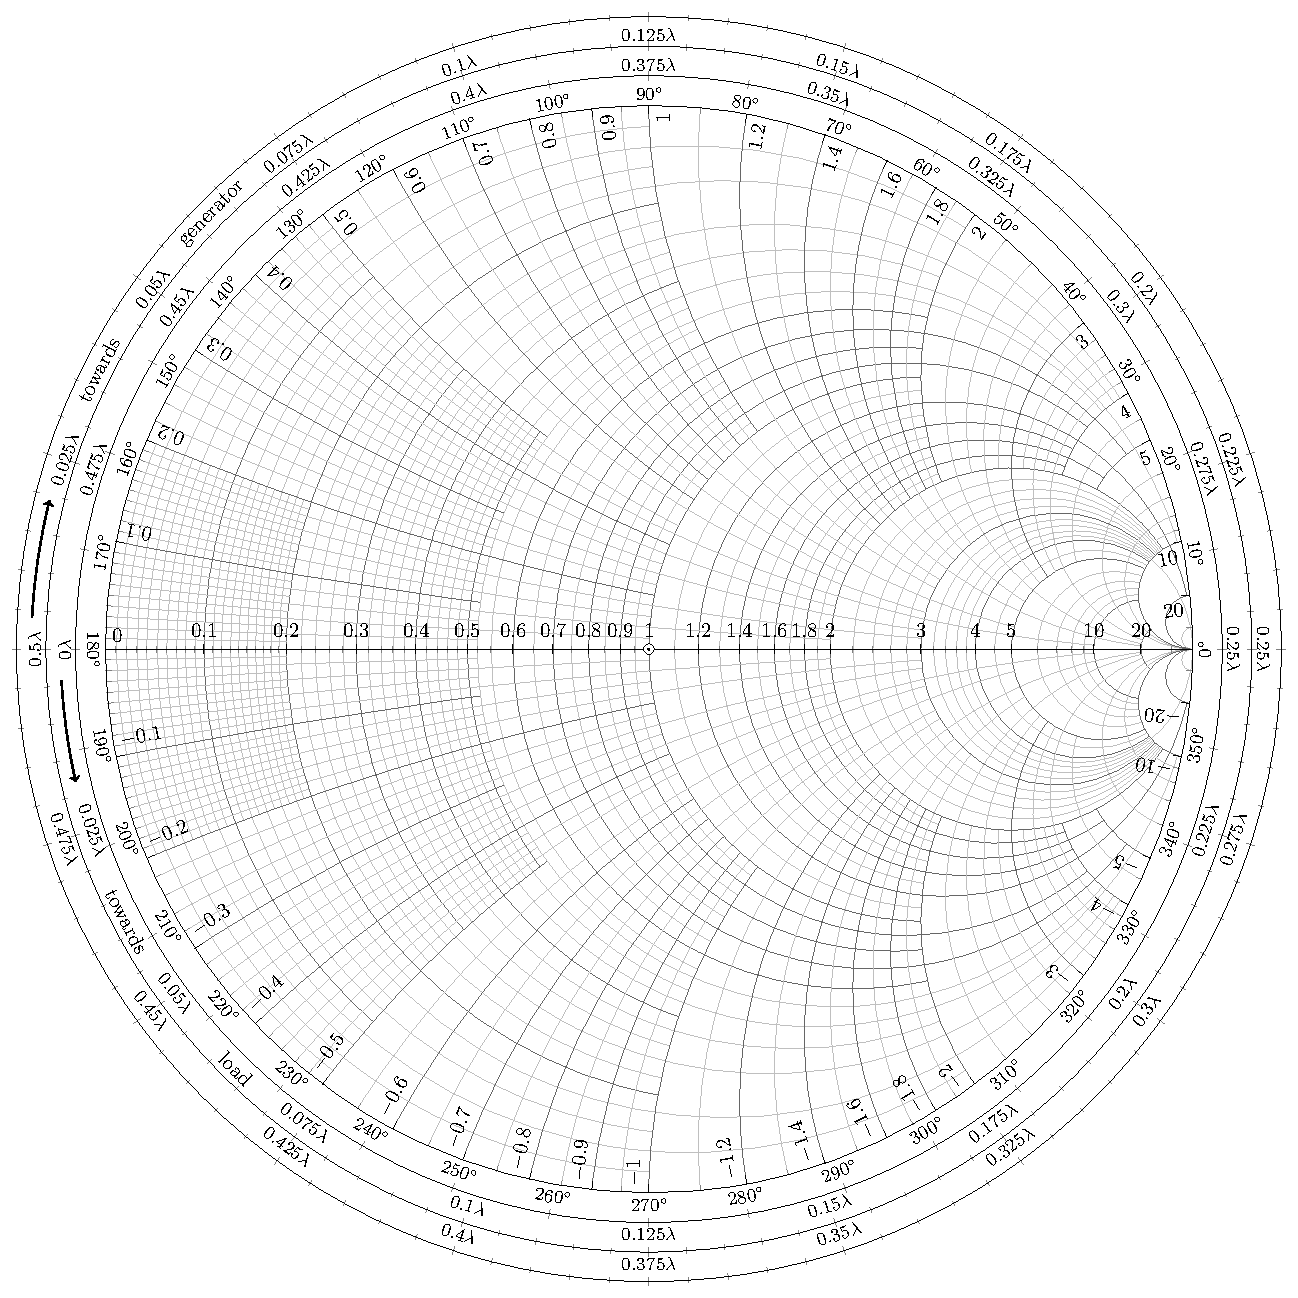
\includegraphics[width=.7\textwidth]{smith.pdf}
    \end{figure}
\end{frame}


\begin{frame}
    \frametitle{Why Smith Chart}
    \begin{outline}
        \1 Developed by P Smith in 1939
        \1 To this day, it is an integral part of microwave circuit design
        \1 Provides a tool to visualise the transmission line phenomena such as impedance matching
        \1 \textcolor{red}{It is simply a polar plot of the reflection coefficient, $\Gamma$}
    \end{outline}
\end{frame}

\begin{frame}
    \frametitle{Navigating the Smith Chart}
    \begin{outline}
        \1 In polar coordinates, $\Gamma = |\Gamma| \e^{\j \theta}$
        \1 We plot the magnitude as a radius $(|\Gamma| \le 1)$ from the centre
        \1 The angle $\theta$ ranges from $\SI{-180}{\degree}$ to $\SI{180}{\degree}$
        \1 \textcolor{red}{The origin} or the centre of the Smith chart is the ideal, matched point.
    \end{outline}
    \begin{figure}[htbp]
        \centering
        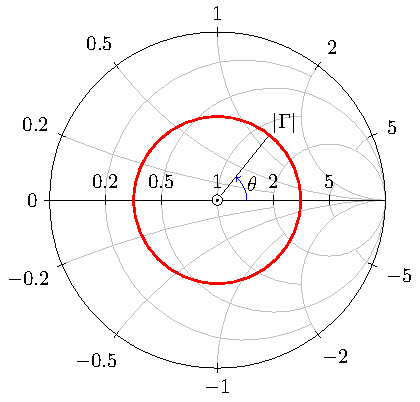
\includegraphics[width=.5\textwidth]{smith_simple_gamme.pdf}
        %   \caption{$\Gamma$ plotted on the Smith chart }
    \end{figure}
\end{frame}

\begin{frame}
    \frametitle{Plotting Impedances}
    For lossles TLs, the \textit{normalised} load impedance at $l = 0$ is a complex number:
    \begin{align*}
        z_L  = \frac{Z_L}{Z_0} & = \frac{1 + |\Gamma|\e^{\j \theta}}{1 - |\Gamma|\e^{\j \theta}}
    \end{align*}
    Treating $\Gamma = \Gamma_r + \j \Gamma_i$, the real and imaginary parts of $z_L$ are:
    \begin{align*}
        r_{L} & = \frac{1-\Gamma_{r}^{2}-\Gamma_{i}^{2}}{\left(1-\Gamma_{r}\right)^{2}+\Gamma_{i}^{2}} \\
        x_{L} & = \frac{2 \Gamma_{i}}{\left(1-\Gamma_{r}\right)^{2}+\Gamma_{i}^{2}}
    \end{align*}
    which can be written as two equations of circles:
    \begin{align*}
        \left(\Gamma_{r} - \frac{r_{L}}{1+r_{L}}\right)^{2} + \Gamma_{i}^{2}      & = \left(\frac{1}{1+r_{L}}\right)^{2} \tag{Resistance Circle} \\
        \left(\Gamma_{r}-1\right)^{2}+\left(\Gamma_{i}-\frac{1}{x_{L}}\right)^{2} & =\left(\frac{1}{x_{L}}\right)^{2} \tag{Reactance Circle}
    \end{align*}
\end{frame}

\begin{frame}
    \frametitle{The Resistance and Reactance Circles}
    \begin{outline}
        \1 Lets look at some examples
        \2 Taking $r_L = 1$ and lets plot in the $\Gamma_r ,\Gamma_i$ plane
        \2 But first, the equation for the resistance circle is:
    \end{outline}
    \begin{align*}
        \left(\Gamma_{r} - \frac{1}{1+1}\right)^{2} + \Gamma_{i}^{2} & = \left(\frac{1}{1+1}\right)^{2}
    \end{align*}
    \begin{figure}[h]
        \centering
        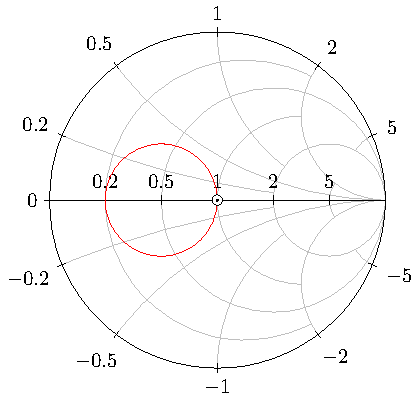
\includegraphics[width=.4\textwidth]{smith_resistance.pdf}
    \end{figure}
\end{frame}

\begin{frame}
    \frametitle{The Resistance and Reactance Circles}

    \begin{outline}
        \1 Now the reactance circle where we take $z_L = \j 1 \implies x_L = 1$
        \1 The reactance circle equation becomes:
    \end{outline}
    \begin{align*}
        \left(\Gamma_{r}-1\right)^{2}+\left(\Gamma_{i}-1\right)^{2} & = 1
    \end{align*}
    \begin{figure}[h]
        \centering
        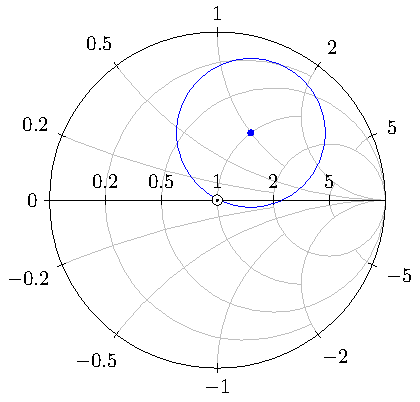
\includegraphics[width=.4\textwidth]{smith_reactance_circle.pdf}
    \end{figure}
    The top half is the \textit{inductive} region and the bottom half is the \textit{capacitive} region.
\end{frame}

\begin{frame}
    \frametitle{Plotting Impedance}
    \begin{columns}[T] % align columns
        \begin{column}{.4\textwidth}
            \begin{outline}
                \1 We normally normalise the impedance to $\SI{50}{\ohm}$.
                \1 However, the chart can be used for any value.
                \1 \textcolor{green}{$z_{L,1} = 0.4 + \j 0.7$}
                \1 \textcolor{red}{$z_{L,2} = 2 $}
                \1 \textcolor{blue}{$z_{L,3} = 3 - \j 2$}
                \1 \textcolor{orange}{$z_{L,4} = 0.2 - \j 0.2$}
            \end{outline}
        \end{column}
        \begin{column}[T]{.6\textwidth}
            \begin{figure}
                \centering
                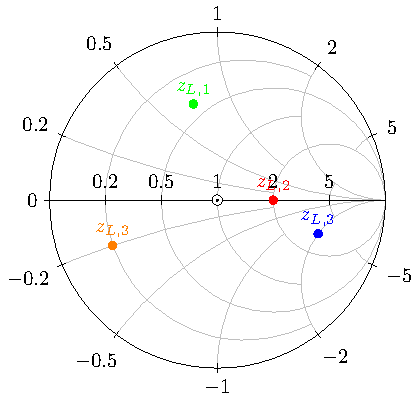
\includegraphics[width=1\textwidth]{smith simple impedances.pdf}
            \end{figure}
        \end{column}%
    \end{columns}
\end{frame}

\begin{frame}
    \frametitle{Travelling on the Smith Chart}
    \begin{columns}{T}
        \begin{column}{.4\textwidth}
            \begin{outline}
                \1 Travelling along a transmission line is equivalent to \textcolor{red}{rotation} along a circle in the Smith chart
                \1 On the Smith chart, different scales labels are provided that tell us which direction we need to consider
            \end{outline}
        \end{column}


    \begin{column}[]{.6\textwidth}
        \begin{figure}[H]
            \centering
            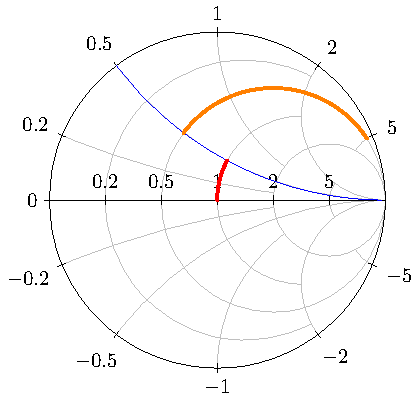
\includegraphics[]{smith_example.pdf}

        \end{figure}
    \end{column}
\end{columns}
\end{frame}
% \end{frame}
\end{document}
